\documentclass[a4paper,10pt]{article}
\usepackage{amsmath}
\usepackage{graphicx}
\usepackage{verbatim}
\usepackage[latin1]{inputenc}
\usepackage{fancyvrb}
\DefineVerbatimEnvironment{code}{Verbatim}{fontsize=\small}
\DefineVerbatimEnvironment{example}{Verbatim}{fontsize=\small}

% Shortcuts for including equations
\newcommand{\beq}{\begin{equation}}
\newcommand{\eeq}{\end{equation}}
\def\i{\hat{i}}
\def\j{\hat{j}}
\def\k{\hat{k}}

% Document formatting
\setlength{\parindent}{0mm}
\setlength{\parskip}{1.5mm}

% Hyper refs
\usepackage[colorlinks]{hyperref}

\usepackage{listings}
\lstset{language=python}
\lstset{basicstyle=\ttfamily\tiny}
\lstset{frame=single}
\lstset{stringstyle=\ttfamily}
\lstset{keywordstyle=\color{red}\bfseries}
\lstset{commentstyle=\itshape\color{blue}}
\lstset{showspaces=false}
\lstset{showstringspaces=false}
\lstset{showtabs=true}
\lstset{breaklines}
\lstdefinestyle{prt}{frame=none,basicstyle=\ttfamily\small}

\newcounter{subproject}
\renewcommand{\thesubproject}{\number{subproject}}
\newenvironment{subproj}{
\begin{description}
\item[\refstepcounter{subproject}(\thesubproject)]
}{\end{description}}

%------------------------------------------------------------
\begin{document} 
{\huge\bf Ast1100 Oblig 6}
\newline Thomas Haaland
\section{}
Skal finne ut hvor lang tid det tar mellom hver gang lyset treffer speilene.
Mellom hvert tikk skal lyset reise $L_0$ meter. Bruker derfor veiformelen

\begin{figure}
 \centering
 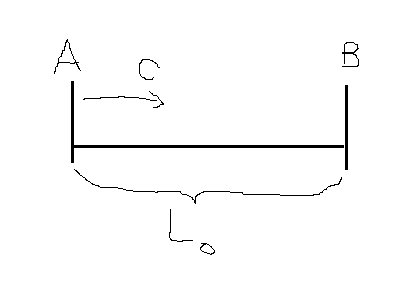
\includegraphics[scale=0.5]{Oppg1.png}
 \label{fig: Oppg1}
 \caption{Lyset reiser fra A til B, med lysfarten c.}
\end{figure}

\beq
c=\frac{s}{t}
\eeq 
der $c$ er lysfarten i x-retning, $s=L_0$ er strekningen lyset skal reise, og $t$ er tiden det tar. F�r dermed

\beq
t=\frac{s}{c}=\frac{L_0}{c}
\eeq

$\frac{L_0}{c}$ er tiden det tar for lyset � reise fra event A til B. 

\section{}
Skal beskrive hendelsene A, B, C. Normaliserer slik at alt blir uttrykt i meter: $v=\frac{v_{norm}}{c}$, $t=t_{norm}\times c$ der $v_{norm}$ og $t_{norm}$ er fart og tid i det umerkede systemet f�r normalisering. Det merkede systemet beveger seg med konstant hastighet $v$ mot �kende $x$. 

\begin{figure}
 \centering
 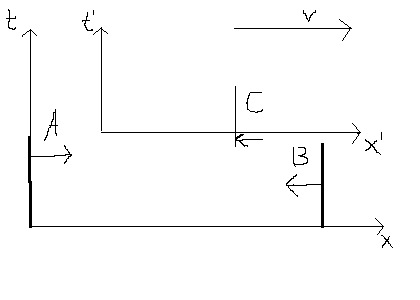
\includegraphics[scale=0.5]{Oppg2.png}
 \label{fig: Oppg2}
 \caption{Det merkede koordinat systemet beveger seg mot st�rre x i hastigheten $v$. Tre hendelser: A, B, C. Hendelsen A er n�r lyset forlater venstre vegg. Hendelse B er n�r lyset blir reflektert av h�yre vegg. Hendelse C er n�r lyset, p� vei tilbake igjen fra h�yre vegg er i $x^{'}=0m$. }
\end{figure}

{\bf A}

$x_A=0m$

$t_A=0m$

$x_A^{'}=0m$

$t_A^{'}=0m$

{\bf B}

$x_B=L_0$

$t_B=L_0$

$x_B^{'}=x_B^{'}$

$t_B^{'}=t_B^{'}$

{\bf C}

$x_C=vt_B$

$t_C=t_B$

$x_C^{'}=0m$

$t_C^{'}=t_C^{'}$

\section{}
Skal skrive ut romtidsintervallet $\Delta s_{AB}=\Delta s_{AB}^{'}$:

\beq
L_0^2-L_0^2=(t_B^{'})^2-(x_B^{'})^2
\eeq

som impliserer
\beq
t_B^{'}=x_B^{'}
\eeq

Siden lyset beveger seg med lyshastigheten er $v=\frac{v_{norm}}{c}=1$ er forlytningen i tid like stor som forflytningen i rom, og dermed $x_B^{'}=t_B^{'}$. Dette siden $\frac{\Delta x}{\Delta \tau}=1$, der $\tau=t_B$ er egentid for lyset. Dette f�lger av lyshastigheten siden $v=\lim_{\Delta \tau \to 0}\frac{\Delta x}{\Delta \tau}=1$ og da m� $\Delta x = \Delta \tau$.

\section{}
Skal skrive ut $\Delta s_{AC}= \Delta s_{AC}^{'}$.

\beq
\Delta s_{AC}=\Delta s_{AC}^{'}
\eeq
\beq
(t_B)^2-(vt_B)^2=(t_C)^2
\eeq
\beq
L_0\sqrt{1-v^2}=t_C^{'}
\eeq
\beq
t_C^{'}=\frac{L_0}{\gamma}
\eeq
Som var det vi skulle vise.

\section{}
Skal skrive ut tidrom intervallet $\Delta s_{BC}= \Delta s_{BC}^{'}$

\beq
\Delta s_{BC}= \Delta s_{BC}^{'}
\eeq
\beq
(L_0-L_0)^2-(vL_0-L_0)^2=(t_C^{'}-t_B^{'})^2-(t_B^{'})^2
\eeq
\beq
-L_0(v^2-2v+1)=\left(\frac{L_0}{\gamma}-t_B^{'}\right)^2-t_B^{'}
\eeq
\beq
-L_0(v^2-2v+1)=\left(\frac{L_0^2}{\gamma ^2}-2t_B\frac{L_0}{\gamma}+(t_B^{'})^2-(t_B^{'})^2\right)
\eeq
\beq
-L_0^2(v^2-2v+1)-L_0^2(1-v^2)=-2t_B^{'}\frac{L_0}{\gamma}
\eeq
\beq
t_B^{'}=\frac{\gamma L_0^2(2-2v)}{2L_0}
\eeq
\beq
t_B^{'}=\gamma L_0(1-v)
\eeq

Som var det vi skulle vise.
\end{document}
